\documentclass[]{jsarticle}

\usepackage[dvipdfmx]{graphicx}
\usepackage{listings,jlisting}
\usepackage{here}
\usepackage{txfonts}
\AtBeginDocument{\RequirePackage{lmodern, times}}

\lstset{%
  language={Python},
  basicstyle={\small},%
  identifierstyle={\small},%
  commentstyle={\small\itshape},%
  keywordstyle={\small\bfseries},%
  ndkeywordstyle={\small},%
  stringstyle={\small\ttfamily},
  frame={tb},
  breaklines=true,
  columns=[l]{fullflexible},%
  numbers=left,%
  xrightmargin=0zw,%
  xleftmargin=3zw,%
  numberstyle={\scriptsize},%
  stepnumber=1,
  numbersep=1zw,%
  lineskip=-0.5ex%
}

\begin{document}
\title{A4988をMOSFET代わりに使うハックのアイディア}
\author{青木翔平}
\date{28, Jul 2015}
\maketitle

\section{発生した問題}
以下の問題が発生した。
\begin{itemize}
\item 買ったMOSFETが動かない
\item 12V流しても24V流しても3V程度しかソースに出てこない
\item ACアダプタのDIP基板に挿したら極性が変わるという謎の問題もあるけどここでは別の話
\end{itemize}

エジソンプラザで買ったMOSFET(2SK352)のグラフを図\ref{2sk352}に示す。
\begin{figure}[htbp]
\centering
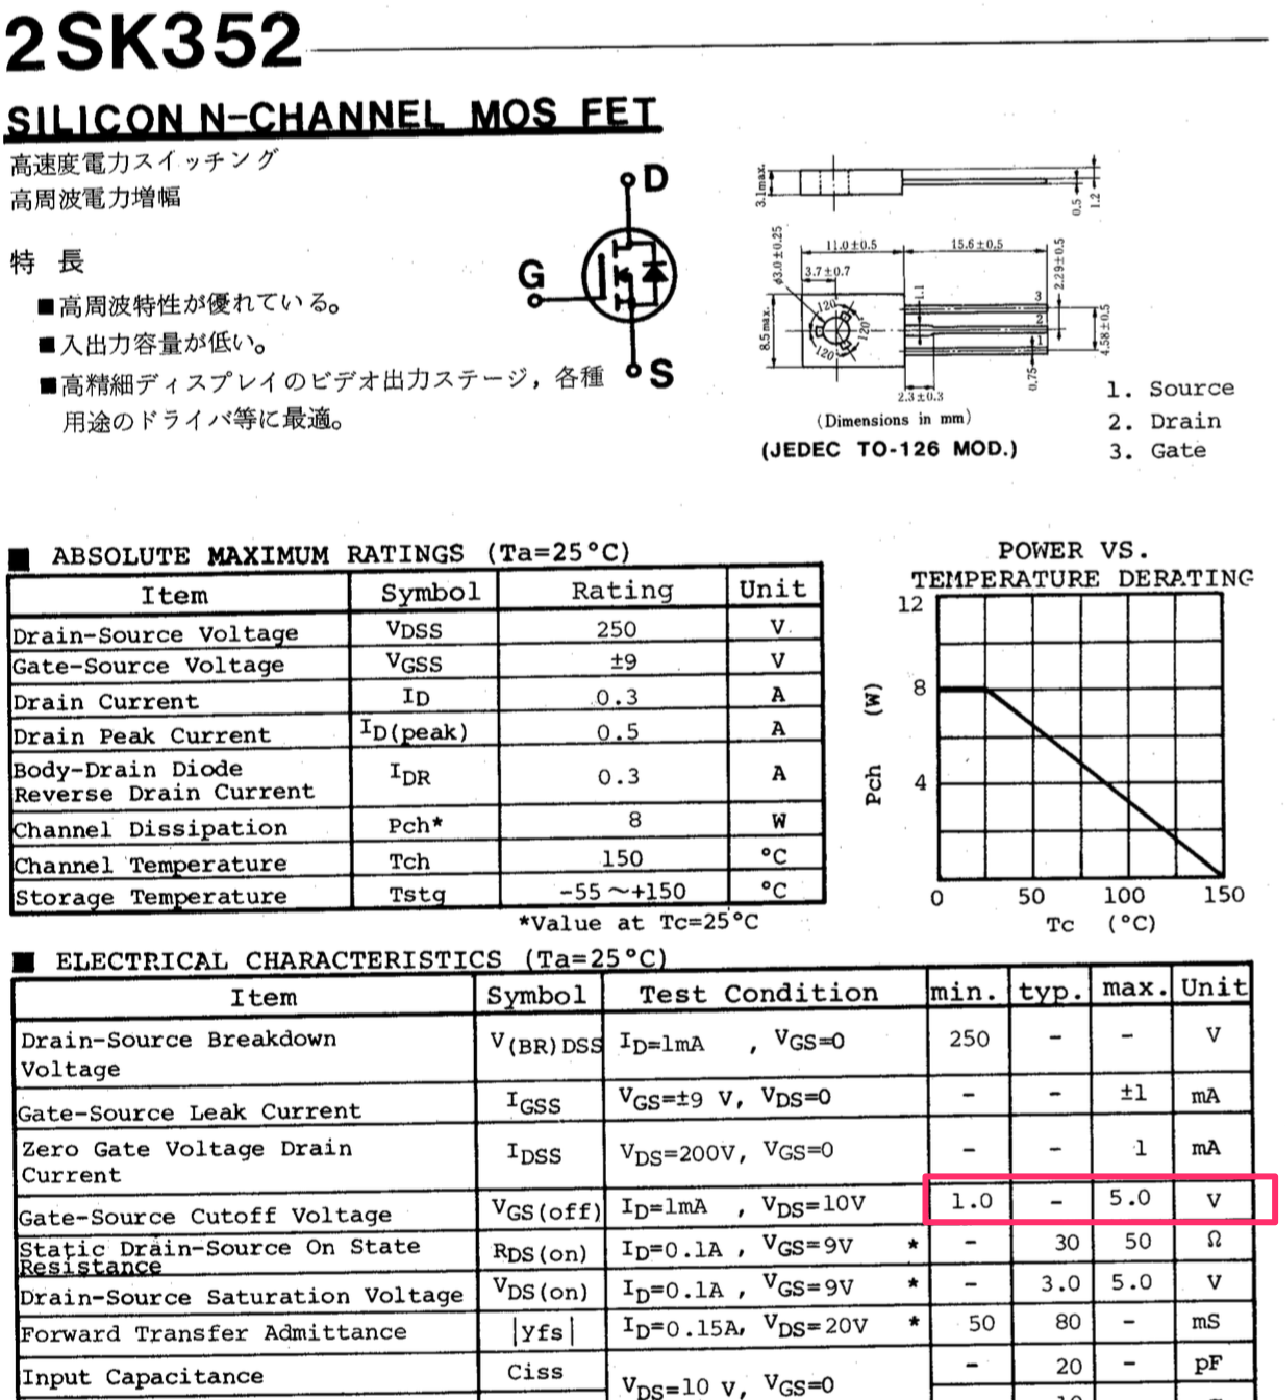
\includegraphics[width=130mm]{./image/2sk352.pdf}
\caption{2SK352のデータシート}
\label{2sk352}
\end{figure}

\section{ステッピングモータのドライバのハック}
A4988はstep信号とdir信号で駆動される一般的なステッピングモータドライバである。この出力波形はマイクロステップ駆動の有無で変わってくるが、step信号のパルスに応じて正弦波を出力するという特性を持つ。例として図\ref{microstep}に16マイクロステップ駆動時の出力波形を示す。

\begin{figure}[htbp]
\centering
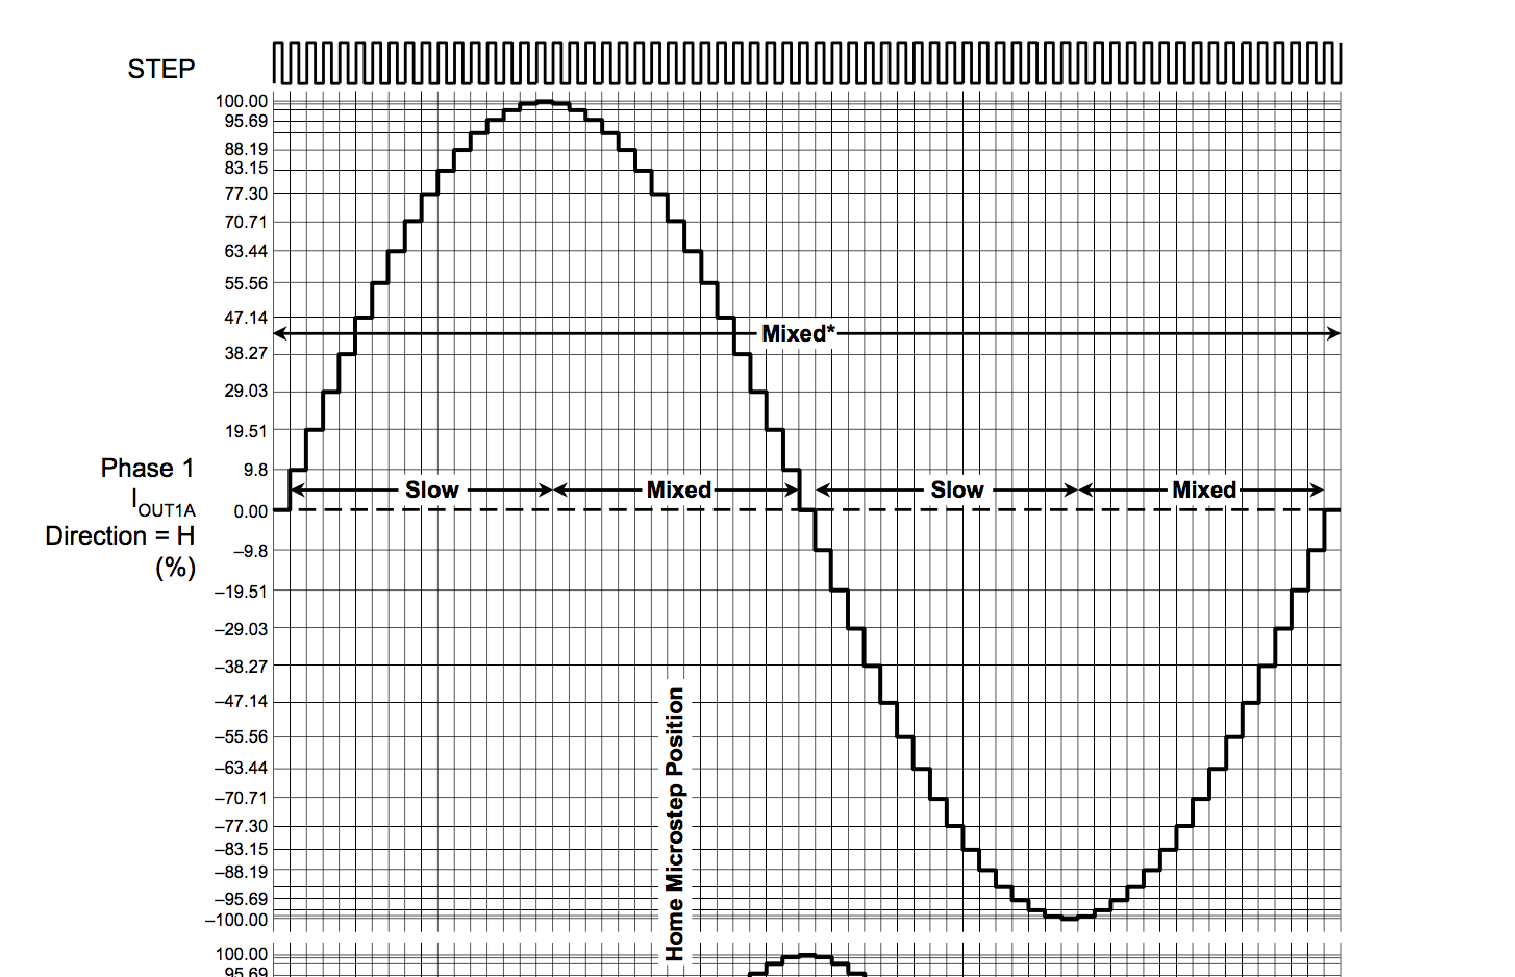
\includegraphics[width=130mm]{./image/16step.pdf}
\caption{16マイクロステップ駆動時の出力波形}
\label{microstep}
\end{figure}

本アイディアは24Vの入力をA4988に加えたとき、出力される正弦波をコンデンサで平滑化してすることで常に12V以上の出力電圧を得てやるという意図である。図\ref{namashi}にこのアイディアを示す。

\begin{figure}
\centering
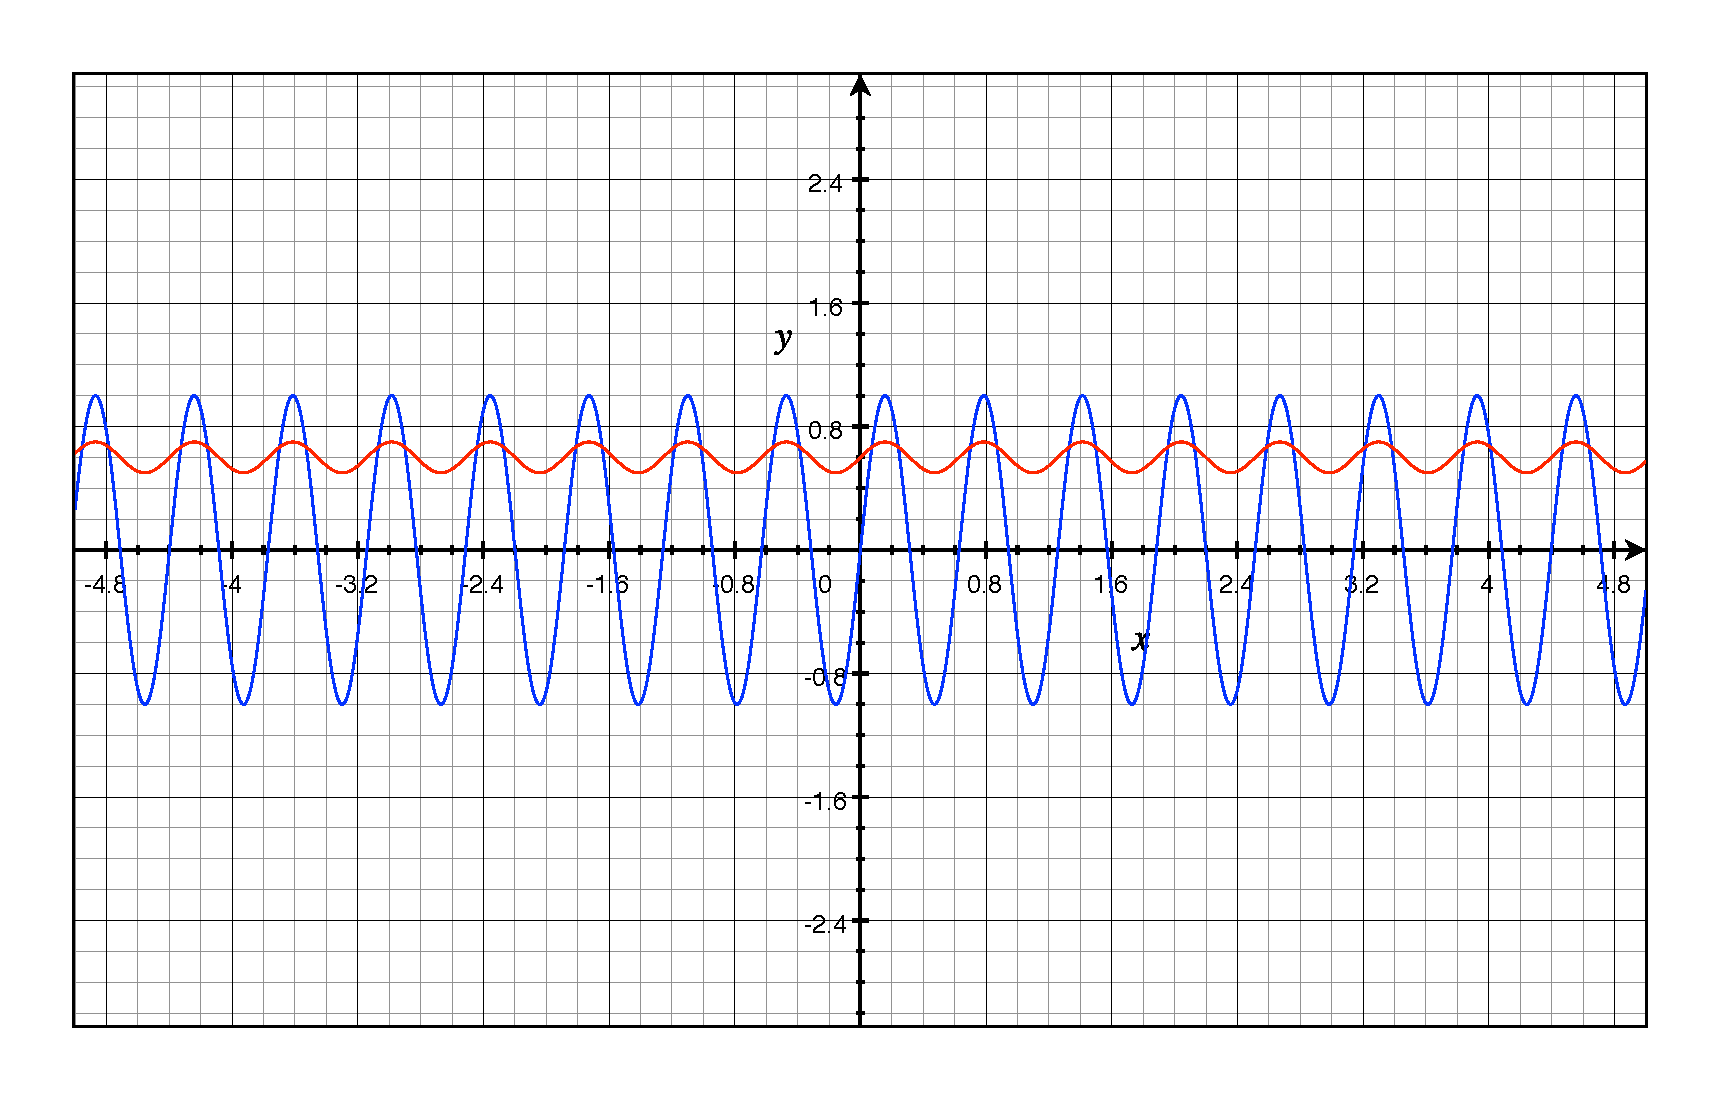
\includegraphics[width=130mm]{./image/namashi.pdf}
\caption{正弦波出力(青線)をコンデンサで平滑して所望の出力(赤線)を得たい}
\label{namashi}
\end{figure}


\section{RC回路の利用}
問題は正弦波入力に対してコンデンサで平滑可能かという点なので、単純のためにRC回路の正弦波入力に対するRC回路の過渡応答を調べる。

RC回路を図\ref{rccircuit}に示す。

\begin{figure}
\centering
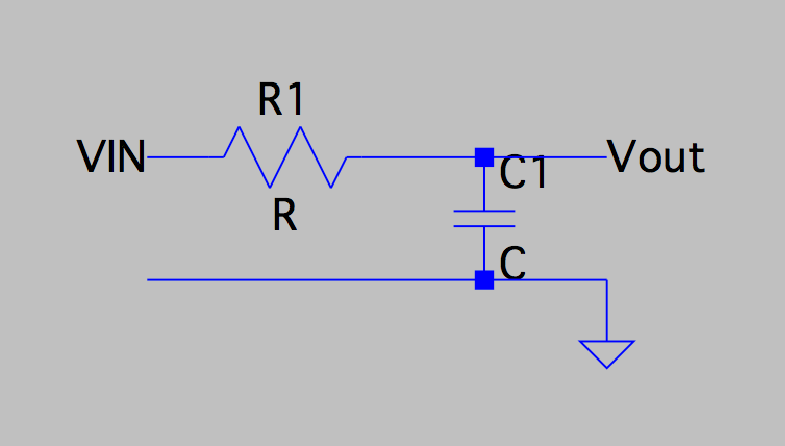
\includegraphics[width=100mm]{./image/rccircuit.pdf}
\caption{RC回路}
\label{rccircuit}
\end{figure}

キルヒホッフの法則と回路方程式から、以下が成り立つ。

\begin{eqnarray*}
v_{i} - v_{o} = i R \\
i = C \cdot \frac{d v_{0}}{dt}
\end{eqnarray*}

両式から$i$を削除して、

\begin{equation}
v_{i} - v_{0} = CR \cdot \frac{d v_{0}}{dt} \label{circuit}
\end{equation}

式(\ref{circuit})をラプラス変換して
\begin{equation}
 V_{i}(s) - V_{o}(s) = CR \cdot sV_{o}(s)
\end{equation}

伝達関数は、
\begin{equation}
 G(s) = \frac{V_{o}(s)}{V_{i}(s)} = \frac{1}{cR s+1} \label{tf}
\end{equation}

$v_{i}$に正弦波として$v_{i} = f(t) = \alpha sin (\omega t)$を与えた時の過渡応答は、式(\ref{tf})の伝達関数に正弦関数のラプラス変換$F(s)$を畳み込んで逆ラプラス変換することで求められる。

\begin{eqnarray*}
G(s)F(s) & = & \frac{1}{CRs+1} \cdot \frac{1}{s^{2}+\omega^{2}} \\
             & = & \frac{1}{CR s^{3}+s^{2}+cs\omega^{2}s+\omega^{2}} \\
             & = & \frac{1}{CR} \cdot \frac{1}{\left( s+\frac{1}{CR} \right)\left( s+i\omega \right)\left( s - i\omega\right)} \\
             & = & \frac{1}{CR} \cdot \left( s - \frac{1}{CR} \right) \cdot \frac{1}{s^{2} - \left( \frac{1}{CR} \right) ^{2}} \cdot \frac{1}{s^{2}+\omega^{2}} \\
             & = & \frac{1}{CR} \left( s - k \right) \cdot \left( \frac{1}{s^{2}-k^{2}} - \frac{1}{s^{2}+\omega^{2}} \right) \cdot \frac{1}{\omega^{2} - k^{2}} \\
             & = & \frac{1}{CR} \left( s - k \right) \cdot \left( \frac{1}{s^{2}-k^{2}} - \frac{1}{s^{2}+\omega^{2}} \right) \cdot \frac{1}{\omega^{2} - k^{2}} \\
             & = & \frac{1}{CR} \left( \frac{1}{s+k} - \frac{s-k}{s^{2}+\omega^{2}}\right) \cdot \frac{1}{\omega^{2} - k^{2}} \\
             & = & \frac{k}{\omega^{2}-k^{2}}\left( \frac{1}{s+k} - \frac{s}{s^{2}+\omega^{2}} + \frac{k}{s^{2}+\omega^{2}}\right)
\end{eqnarray*}

ラプラス逆変換して、
\begin{eqnarray*}
v_{o}(t) = L^{-1}[G(s)F(s)] = \frac{k}{\omega^{2}-k^{2}}\left( e^{-kt} + cos(\omega t) + k sin(\omega t)\right)
\end{eqnarray*}

$R = 1 [k \Omega], C=1,10,100,100[\mu F] $で計算するコードをソースコード\ref{code}に示す。

\begin{lstlisting}[caption=正弦波入力に対する応答解析,label=code]
#!/usr/bin/env python
#-*- coding:utf-8 -*-

from pylab import *

C_array = [1.0*10**-6,10.0*10**-6,100.0*10**-6,1000.0*10**-6] #[F]
R = 1000.0 #[Ω]
f = 100 # [Hz], 100 pulse per sec
omega = f / (2.0*pi) #[rad/s]

yscale('log')
for C in C_array:
    response = [] 
    k = 1/(C*R)
    t = arange(0,10,0.001)
    response = k*(omega**2-k**2)*(exp(-1.0*k*t) - cos(omega*t) - k*sin(omega*t))
    plot(t,response)

show()
\end{lstlisting}

出力結果を図\ref{result}に示す。
\begin{figure}
\centering
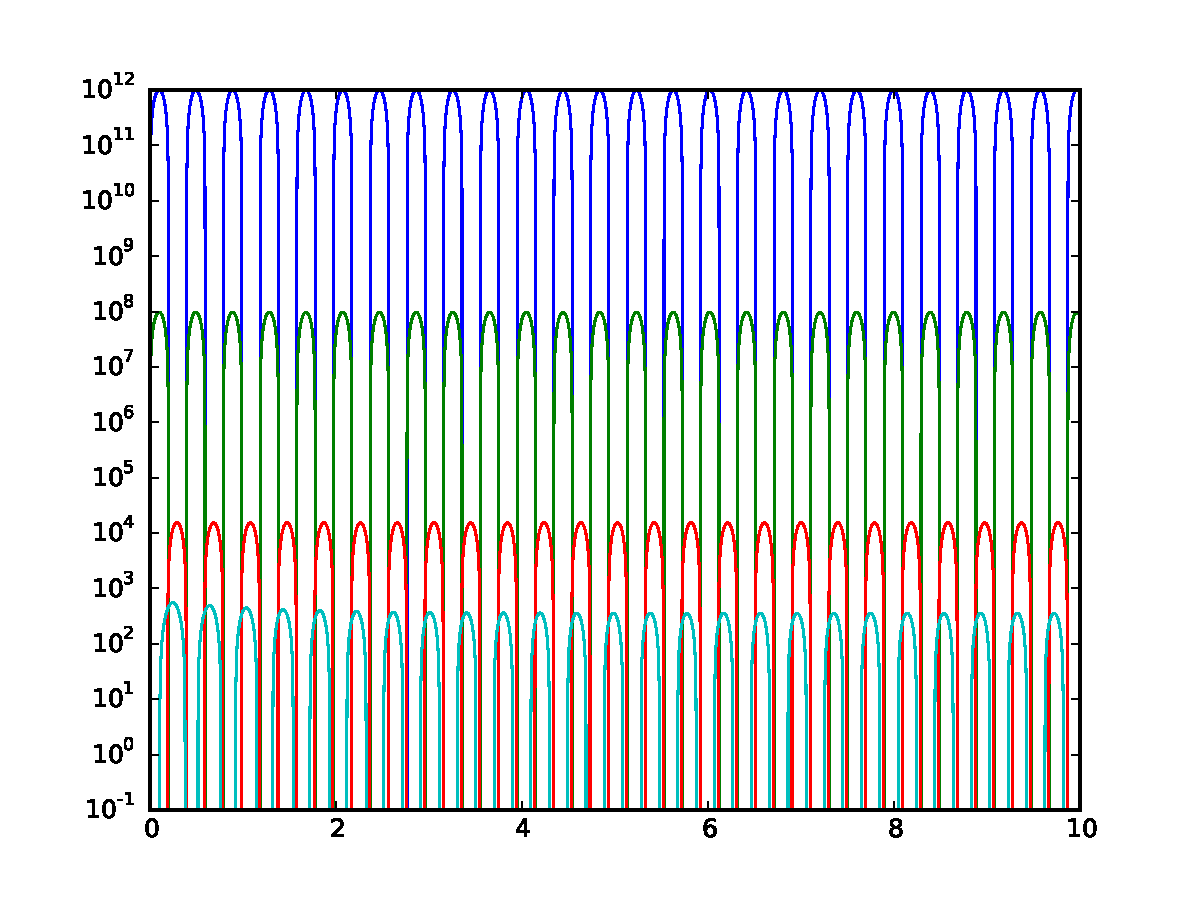
\includegraphics[width=130mm]{./image/result.pdf}
\caption{計算結果}
\label{result}
\end{figure}

図\ref{result}を見る限りでは入力は減衰されていない。

\section{議論}
\begin{itemize}
\item 計算式の見直し
\item パラメータの変更
\end{itemize}

\end{document}
